%!TEX root = ./template-skripsi.tex
%-------------------------------------------------------------------------------
%                            	BAB III
%               		    METODE PENELITIAN
%-------------------------------------------------------------------------------

\chapter{METODE PENELITIAN}

\section{Deskripsi Sistem}
    Sistem bertujuan untuk melakukan penghitungan panjang serta berat objek ikan yang menggunakan
metode`\emph{Harris-Corner Detection} dan`\emph{Gaussian Laplace}. Penelitian berfokus dalam menghasilkan berupa
data hasil panjang dan berat objek ikan. Dataset citra ikan diambil secara langsung menggunakan`\emph{Smartphone} pada sebuah
penangkaran ikan. Kemudian bahasa yang akan digunakan dalam membangun sistem adalah Python versi 3.

Tahapan dalam penghitungan panjang dan berat ikan menggunakan`\emph{Harris-Corner Detection} adalah Pemrosesan Citra,
\emph{Smoothing Gaussian}, Perhitungan gradien, autokorelasi matriks gradien,`\emph{Harris Respons}, melakukan threshold-ing dan`\emph{Non-Maximum Suppression}, menentukan koordinat sudut, perhitungan panjang dan lebar, Penghitungan berat,
dan terakhir adalah mengasosiasikan data.

\section{Perancangan Sistem}
    Pada bagian ini akan membahas tentang proses yang akan dilakukan untuk mengetahui tahapan yang ditempuh
dalam membangun sistem penghitungan berat dan panjang ikan. Tahapan pertama yang dilakukan adalah melakukan`\emph{input} gambar
yang akan dibaca sistem, setelah itu citra akan diproses menggunakan`\emph{Smoothing Gaussian} untuk mengurangi`\emph{noise}. Kemudian perhitungan gradien dilakukan bertujuan untuk menghitung setiap perubahan intensitas yang berada di sekitar titik,
hasil tersebut akan diolah kembali menggunakan autokorelasi matriks gradien, dan dilanjutkan dengan menjalankan`\emph{Harris Respons}.\emph{Harris Respons} bertujuan untuk mengetahui bahwa titik tersebut adalah sebuah sudut, atau sisi berdasarkan pada hasil respon Harris.
Hasil dari Harris akan memasuki tahapan thresholding dan`\emph{non-maximum suppression} untuk memilih sudut maksimum pada area tertentu. Setelah mendapatkan titik yang merupakan sebuah sisi, titik-titik tersebut akan dipilih.
Hasil dari pemilihan tersebut akan digunakan untuk menghitung panjang, lebar, dan berat ikan. Gambaran perancangan sistem yang sederhana terdapat pada gambar~\ref*{Alur Penelitian}

\begin{figure}
    \centering
    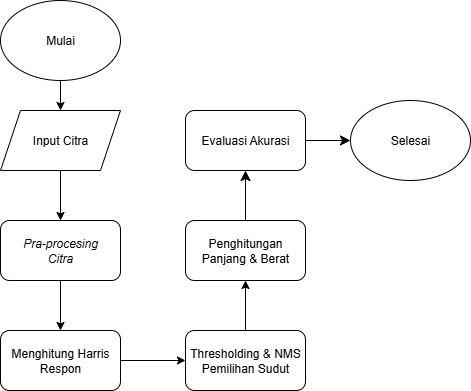
\includegraphics[scale= 0.7]{gambar/Alur Penelitian.png}
    \caption{Alur Penelitian}\label{Alur Penelitian}
\end{figure}

\section{Pra-Processing Citra}
    Pada tahap ini, citra ikan yang akan digunakan sebagai input sistem akan melalui beberapa tahapan pra-processing.
Pra-processing bertujuan untuk mempersiapkan citra agar siap untuk diproses lebih lanjut. Langkah-langkah pra-processing yang dilakukan adalah sebagai berikut:
\begin{enumerate}
    \item Gambar yang akan digunakan berformat jpg atau png, dengan latar belakang yang telah dihilangkan dan digantikan dengan warna solid hitam.  Jenis dataset dapat dilihat pada Gambar~\ref{fig:dataset}.
    \item Proses input citra ke dalam sistem dilakukan menggunakan library`\emph{scikit-image (skimage)} pada bahasa pemrograman Python.\emph{Scikit-image} merupakan library open-source yang digunakan untuk pemrosesan citra digital, menyediakan berbagai fungsi seperti pembacaan, konversi, filtering, segmentasi, dan analisis citra secara efisien. Dengan`\emph{skimage.io.imread}, citra dapat dibaca dan diproses lebih lanjut secara efisien.
    \item Setelah citra berhasil diinput, langkah selanjutnya adalah konversi ke`\emph{grayscale} untuk mempermudah proses pendeteksian sudut agar lebih akurat.
    \item Setelah citra dikonversi ke`\emph{grayscale}, langkah selanjutnya adalah menerapkan`\emph{Gaussian smoothing} untuk mengurangi`\emph{noise} pada gambar.
\end{enumerate}

\begin{figure}
	\centering
	\begin{subfigure}{.3\textwidth}
		\centering
        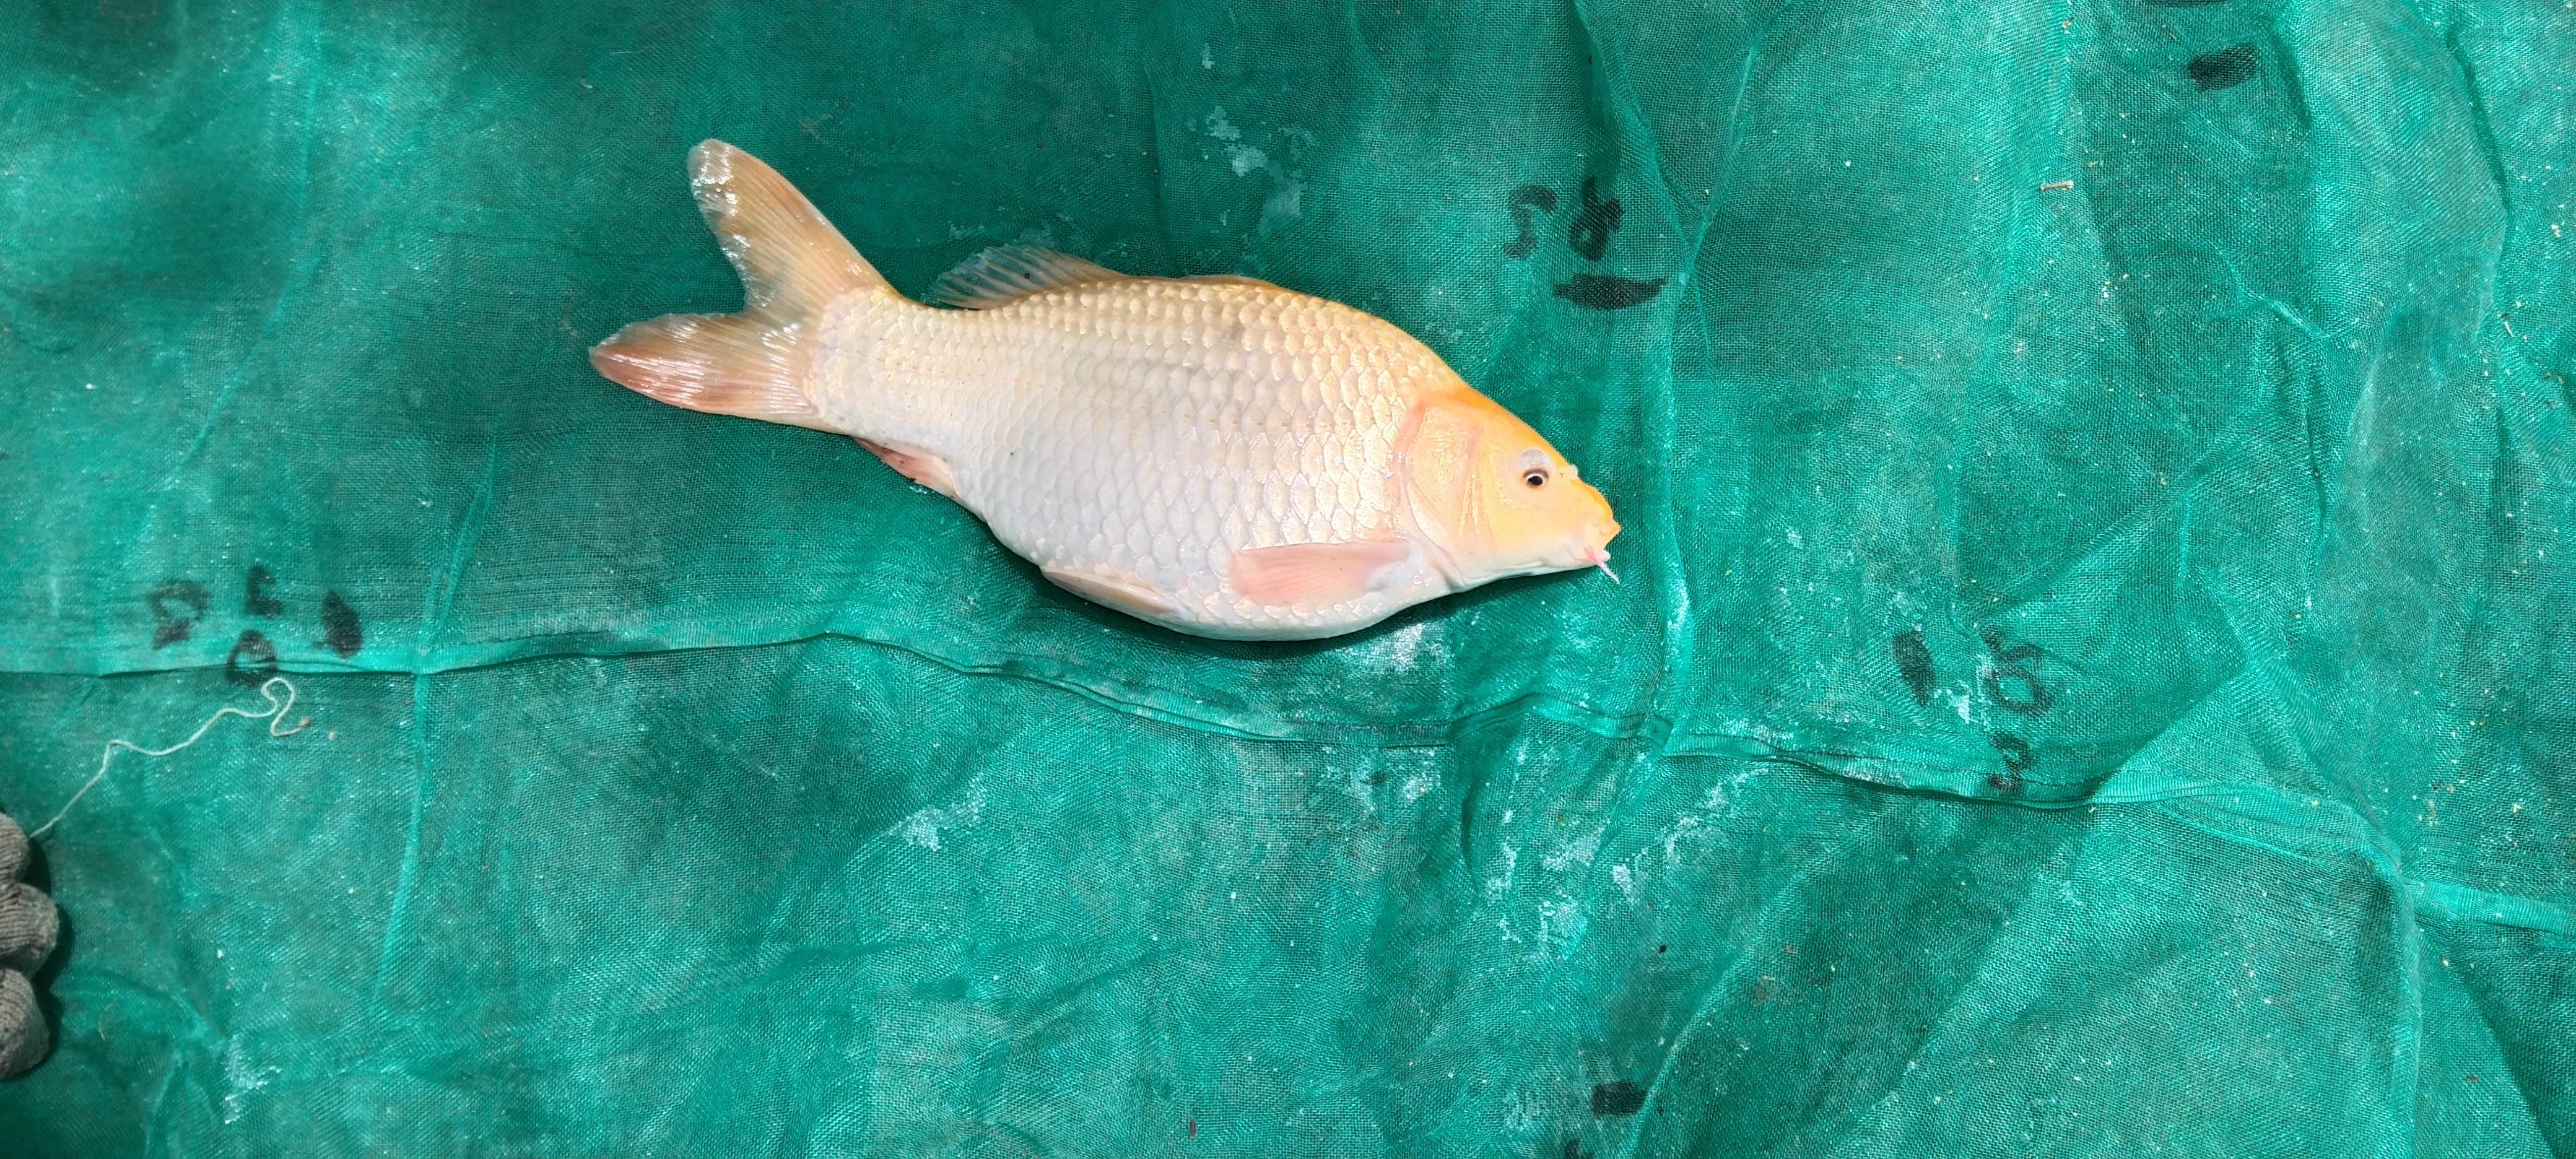
\includegraphics[keepaspectratio, width=3cm]{gambar/IMG_20240121_131125.jpg}
		\caption{Ikan Mas}
	\end{subfigure}
	\begin{subfigure}{.3\textwidth}
		\centering
		\includegraphics[keepaspectratio, width=3cm]{gambar/IMG_20240121_132544.jpg}
		\caption{Ikan lele}
	\end{subfigure} 
	\begin{subfigure}{.3\textwidth}
		\centering
		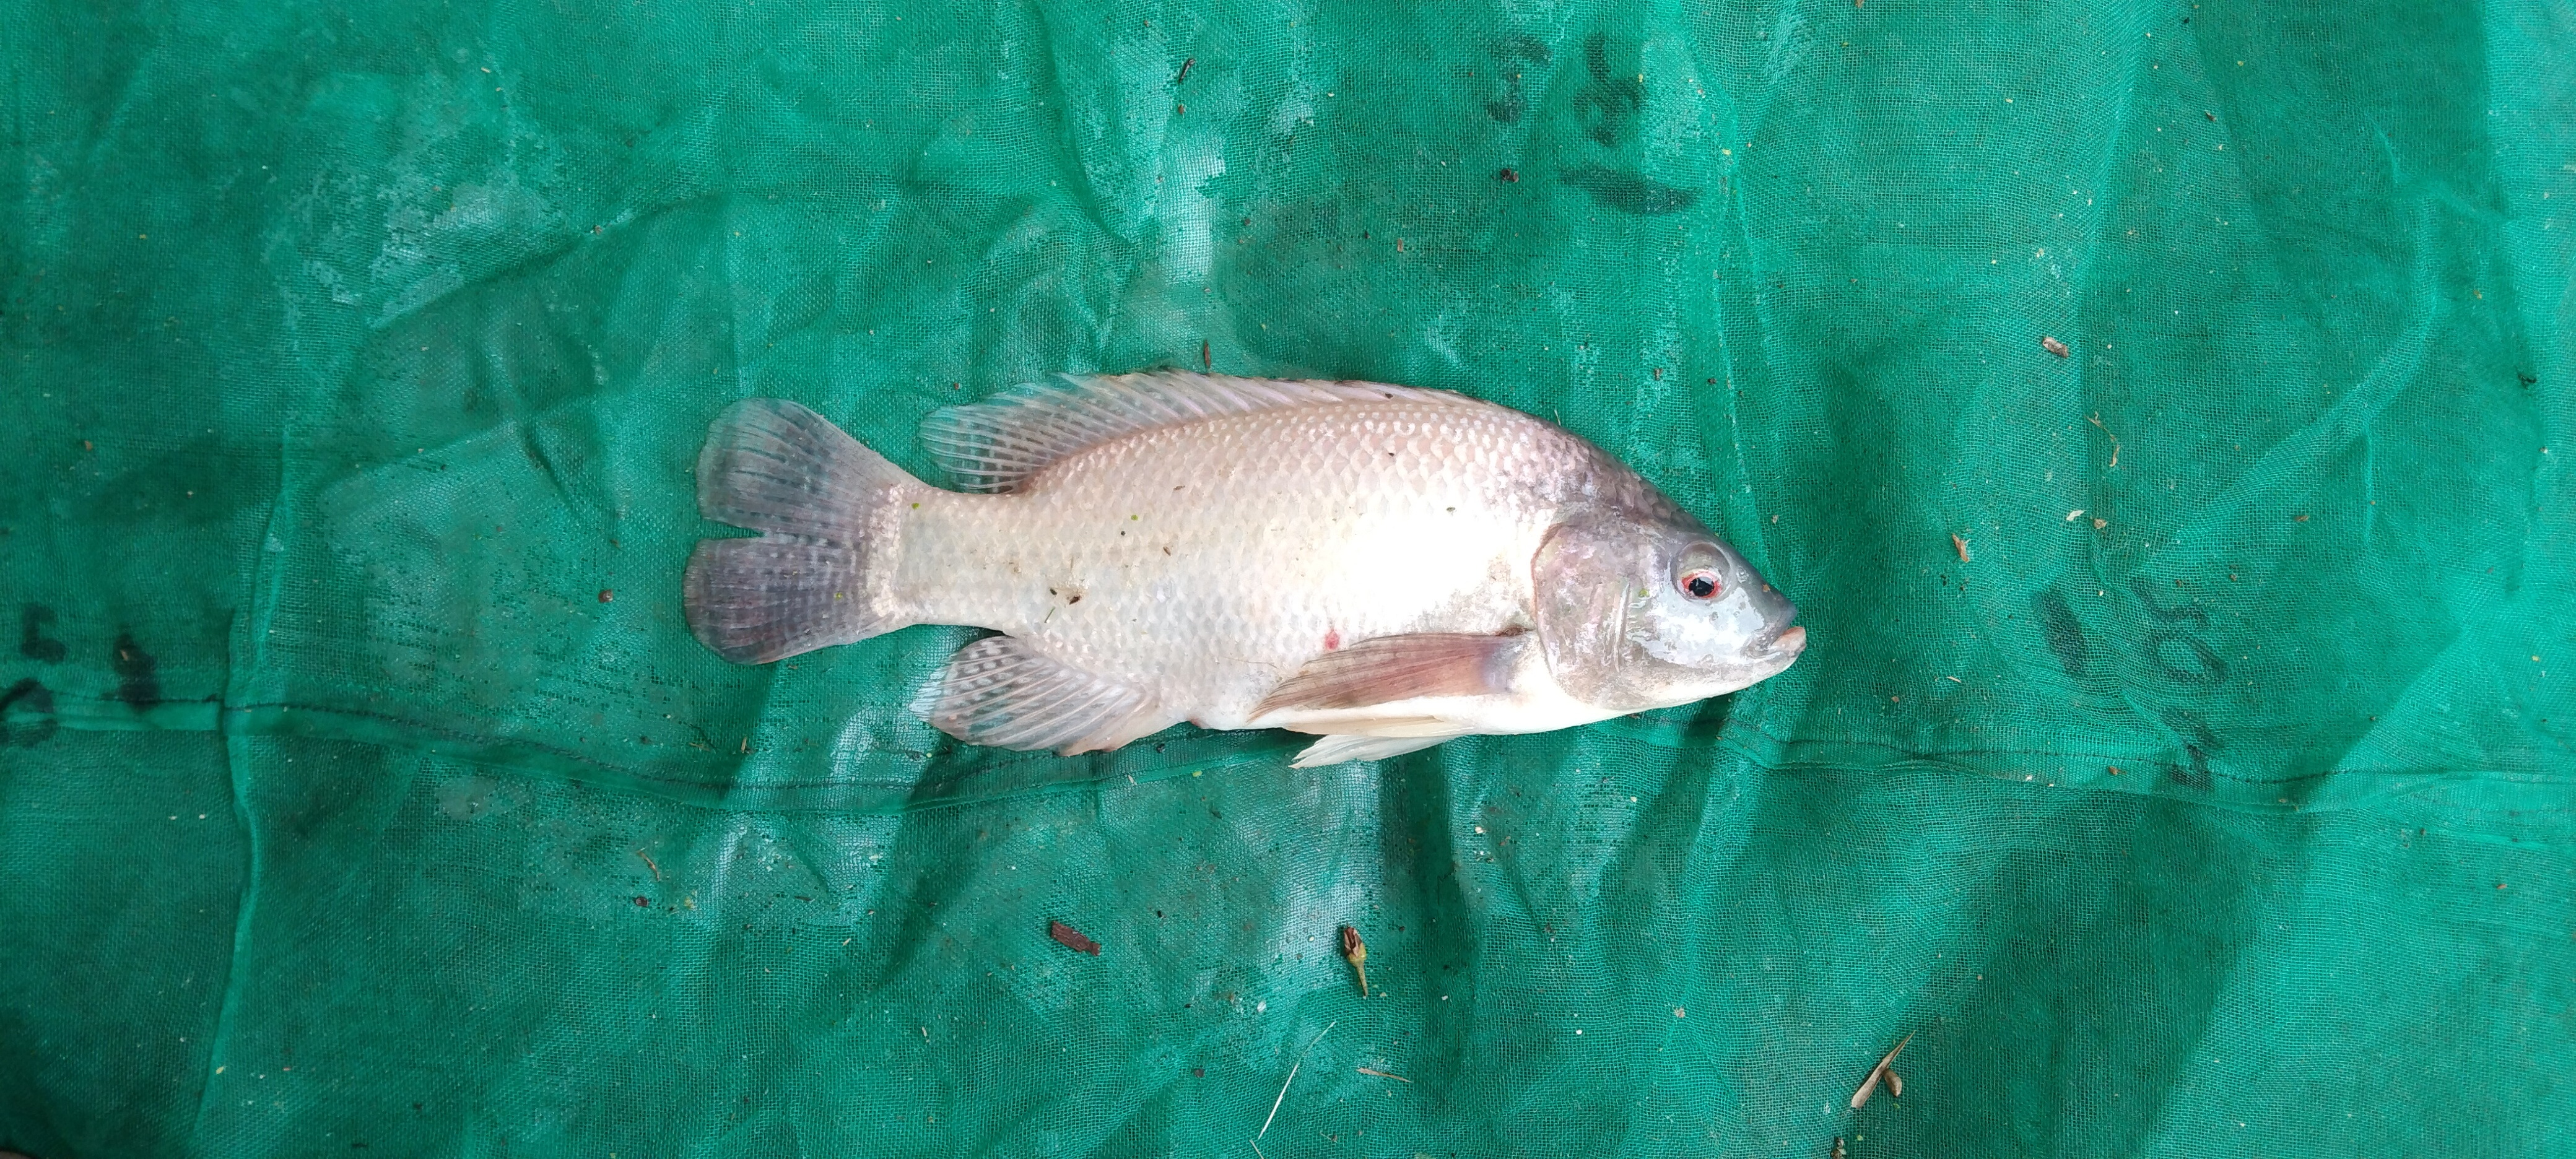
\includegraphics[keepaspectratio, width=3cm]{gambar/IMG_20240121_140044.jpg}
		\caption{Ikan Nila Merah}
	\end{subfigure}
	\caption{Jenis Ikan yang Digunakan}\label{fig:dataset}
\end{figure}

\subsection{Smoothing Gaussian}
   `\emph{Smoothing Gaussian} digunakan untuk mengurangi`\emph{noise} pada gambar sebelum melanjutkan ke perhitungan lebih lanjut.
\emph{Noise} adalah gangguan yang muncul dalam gambar digital yang dapat mengaburkan detail atau informasi penting.`\emph{noise} dapat disebabkan oleh berbagai faktor, seperti kualitas sensor kamera yang rendah, pencahayaan yang buruk, atau kesalahan dalam proses pemindahan data.
Dalam gambar,`\emph{noise} biasanya terlihat sebagai bintik-bintik acak atau intensitas piksel yang tidak diinginkan. Keberadaan`\emph{noise} ini dapat menjadi masalah dalam proses pendeteksian sudut, karena`\emph{noise} dapat menyebabkan munculnya sudut palsu yang tidak sesuai dengan gambar asli.
    
    Langkah pertama dalam`\emph{smoothing Gaussian} adalah membentuk`\emph{Gaussian kernel}. Pemilihan ukuran kernel sangat berpengaruh terhadap hasil`\emph{smoothing}, khususnya pada tingkat kehalusan gambar dan jumlah`\emph{noise} yang berkurang.
Semakin besar kernel yang digunakan, semakin banyak`\emph{noise} yang dihilangkan, tetapi hal ini dapat menyebabkan detail gambar ikut terhapus. Sebaliknya, jika kernel yang digunakan berukuran kecil, detail gambar akan lebih terjaga, tetapi`\emph{noise} mungkin masih tetap ada.
Setelah menentukan ukuran kernel yang akan digunakan kernel dapat dihitung dengan menggunakan persamaan~\eqref{eq:gaussian kernel}.

    Langkah selanjutnya adalah mengaplikasikan kernel pada gambar. Proses ini dilakukan dengan menerapkan kernel secara berulang pada setiap piksel di seluruh gambar.
Namun, sebelum langkah tersebut, gambar perlu di-\emph{padding} terlebih dahulu.`\emph{Padding} adalah proses menambahkan piksel pada tepi gambar sebelum pemrosesan dengan kernel atau model dimulai.
Tujuan dari`\emph{padding} adalah untuk mempertahankan ukuran gambar setelah diterapkannya operasi tertentu, seperti konvolusi. 
Setelah`\emph{padding} diterapkan, konvolusi akan dilakukan dengan menggunakan persamaan~\eqref{eq:konvolusi}. 

\subsection{Perhitungan Gradien}
    Gambar yang telah diperhalus akan dilanjutkan dengan menghitung gradien pada setiap`\emph{pixel}-nya. Tujuan dari penghitungan gradien adalah untuk mengetahui perubahan intensitas pada setiap piksel, yang pada umumnya akan menujukan tepi atau kontur dalam sebuah gambar.
Penghitungan gradien juga memerlukan kernel untuk dapat bekerja, terdapat banyak kernel yang dapat digunakan untuk menghitung gradien, contohnya kernel sobel. 

    Kernel Sobel digunakan untuk menghitung estimasi gradien dengan memberikan bobot yang lebih besar pada piksel tetangga terdekat di sekitar piksel pusat.
Kernel sobel terdiri dari dua matriks \(3 \times 3\), yang bertujuan untuk menghitung gradien pada dua arah yaitu:
 \begin{itemize}
    \item \textbf{Gradien Horizontal} \((G_{x})\): Mengukur perubahan intensitas sepanjang sumbu x.
    \item \textbf{Gradien Vertical} \((G_{y})\): Mengukur perubahan intensitas sepanjang sumbu y.
\end{itemize}Kernel operator sobel dapat dilihat pada persamaan~\eqref{eq:sobel-kernel}. 
Perhitungan gradien juga akan menggunakan rumus~\eqref{eq:konvolusi} tetapi gaussian filter akan diganti dengan kernel sobel horizontal (Gx) dan kernel sobel vertical (Gy).
Maka rumusannya akan seperti berikut:
\begin{equation}
    \begin{aligned}
        G_{x} = S_{x} * I(x)\\ G_{y} = S_{y} * I(x)
    \end{aligned}
\end{equation}


\subsection{Menghitung Second Moment Matriks}
    Setelah hasil dari perhitungan gradien didapatkan, hasil tersebut akan dibuat menjadi matriks kembali dengan rumus~\eqref{eq:SecondMomentMatrix}. Nilai gradien dihitung untuk mendapatkan koefisien matriks autokorelasi. Setelah koefisien didapatkan, koefisien tersebut akan dikonvolusi dengan filter gaussian.
Hasil dari konvolusi digunakan untuk membentuk matriks \(M\) yang akan digunakan untuk perhitungan selanjutnya. Bentuk dari matriks \(M\) sebagai berikut:

\begin{equation*}
    \begin{aligned}
        \Sigma I_{x} = g(\sigma) * G_{x}^2 \\
        \Sigma I_{x}I_{y} = g(\sigma) * G_{x} * G_{y} \\
        \Sigma I_{y} = g(\sigma) * G_{y}^2
    \end{aligned}
\end{equation*}

\begin{equation}
    M = 
    \begin{bmatrix}
        \Sigma I_{x} & \Sigma I_{x}I_{y} \\
        \Sigma I_{x}I_{y} & \Sigma I_{y}
    \end{bmatrix} 
\end{equation}

\subsection{Harris Respon}
    Matriks \(M\) digunakan untuk menghitung respon Harris, menggunakan rumus Harris yaitu:
\begin{equation}
    R(x,y) = Det(M) - k * {trace(M)}^2
\end{equation}
Dimana \(Det(M)\):
\begin{equation*}
    Det(M) = \Sigma I_{x} * \Sigma I_{y} - \Sigma I_{x}I_{y}^2
\end{equation*}
Dan \(trace(M)\) 
\begin{equation*}
    trace(M) = \Sigma I_{x} + \Sigma I_{y}
\end{equation*}

    Dimana \(k = 0.04\). Penggunaan`\emph{Harris-Corner Detection} bertujuan untuk menandai bahwa piksel tersebut adalah sudut atau tidak.

    Nilai respon Harris (\(R\)) menunjukkan seberapa besar kemungkinan suatu piksel merupakan titik sudut pada citra. Jika nilai \(R\) besar dan positif, maka area tersebut memiliki perubahan intensitas yang signifikan ke segala arah dan kemungkinan merupakan sudut (\emph{corner}). Jika nilai \(R\) kecil atau negatif, maka area tersebut cenderung merupakan tepi atau bagian datar. Dengan demikian, perhitungan respon Harris sangat penting untuk membedakan antara sudut, tepi, dan area datar pada citra, sehingga hanya titik-titik yang benar-benar merupakan sudut yang akan dipilih untuk proses selanjutnya.

\subsection{Thresholding dan`\emph{Non-Maximum suppression}}
    Setelah nilai harris didapatkan tahapan langkah selanjutnya adalah melakukan Thresholding.
Thresholding adalah cara untuk memilih hasil deteksi dengan cara menetapkan nilai ambang batas.
Jika nilai harris melebihi dari ambang batas, maka piksel tersebut akan dianggap sebagai potensial sudut kuat, Sebaliknya jika nilai harris lebih kecil maka piksel tersebut akan diabaikan.
Tujuannya supaya mengurangi piksel yang perlu diproses lebih lanjut.
\begin{equation}
    Corner(x,y) = 
    \begin{cases}  
        1 & \text{jika } R(x,y) > T \\ 
        0 & \text{jika } R(x,y) <= T
    \end{cases}
\end{equation}

    Setelah melewati Thresholding, setiap piksel yang telah lolos akan diperiksa kembali dengan`\emph{Non-Maximum Suppression} atau NMS,
NMS bertujuan untuk mengelola kembali piksel yang saling berdekatan satu sama lain. NMS akan memilih piksel pada rentang tertentu, piksel dengan nilai \(R\) terbesar akan terpilih sebagai puncak lokal dan dipertahankan sebagai sudut, dan yang lainnya akan diabaikan.
\begin{equation*}
    NMS(x,y) =
    \begin{cases}
        1 & \text{jika } R(x,y) = MaxLocal R(i,j) \\
        0 & \text{lainnya }
    \end{cases}
\end{equation*}
Dimana`\emph{MaxLocal} \(R(i,j)\) adalah nilai maksimum yang berada di sekitar piksel \((x,y)\).

\subsection{Memilih Piksel}
    Setelah sudut-sudut hasil Thresholding dan NMS diperoleh, langkah selanjutnya adalah memilih piksel-piksel yang akan digunakan sebagai acuan pengukuran panjang dan lebar ikan. Pemilihan titik-titik sudut ini didasarkan pada jarak maksimum antar titik, sehingga diperoleh titik-titik yang mewakili bagian-bagian utama tubuh ikan, seperti ujung kepala (mulut), ujung ekor, sirip atas, dan bagian bawah perut.

    Proses pemilihan dilakukan dengan cara mencari pasangan titik sudut yang memiliki jarak Euclidean terjauh satu sama lain. Rumus jarak Euclidean antara dua titik \((x_1, y_1)\) dan \((x_2, y_2)\) adalah:
\begin{equation}
    d = \sqrt({x_2 - x_1}^2 + {y_2 - y_1}^2)
\end{equation}

    Langkah-langkah pemilihan titik adalah sebagai berikut:
\begin{enumerate}
    \item Hitung jarak Euclidean untuk setiap pasangan titik sudut yang terdeteksi.
    \item Pilih dua titik dengan jarak maksimum sebagai titik ujung (biasanya mewakili mulut dan ekor ikan).
    \item Untuk menentukan titik sirip atas dan bawah, cari dua titik lain yang memiliki jarak maksimum secara vertikal terhadap garis yang menghubungkan dua titik utama (mulut dan ekor).
\end{enumerate}

    Dengan pendekatan ini, pemilihan titik menjadi lebih objektif dan akurat karena didasarkan pada distribusi spasial sudut-sudut hasil deteksi, bukan hanya pada posisi relatif secara manual. Jika jenis ikan memiliki morfologi khusus (misal ikan lele), penyesuaian dapat dilakukan dengan memilih titik-titik yang relevan sesuai bentuk tubuh ikan.
\subsection{Menghitung Panjang dan Berat}
    Setelah titik-titik sudut utama diperoleh dari proses pemilihan piksel, langkah selanjutnya adalah menghitung panjang ikan berdasarkan jarak Euclidean antara dua titik terjauh tersebut. Rumus yang digunakan adalah:
\begin{equation}
    d = \sqrt({x_2 - x_1}^2 + {y_2 - y_1}^2)
\end{equation}
    di mana \((x_1, y_1)\) dan \((x_2, y_2)\) adalah koordinat dua titik sudut terjauh hasil deteksi. Nilai \(d\) ini merupakan panjang ikan dalam satuan piksel.

    Untuk mengonversi panjang dari satuan piksel ke satuan nyata, diperlukan faktor skala. Skala dapat diperoleh dengan dua cara, yaitu menggunakan objek referensi yang diketahui ukurannya dalam gambar, atau berdasarkan resolusi gambar:
\begin{equation*}
    Skala = \frac{\text{Ukuran nyata (cm)}}{\text{Ukuran pada gambar (piksel)}}
\end{equation*}
\begin{equation}
    Panjang\ Nyata = d \times Skala
\end{equation}

    Setelah panjang ikan dalam satuan nyata diketahui, estimasi berat ikan dapat dilakukan menggunakan rumus interpolasi linier berdasarkan data panjang dan berat ikan yang telah diketahui sebelumnya. Rumus interpolasi linier yang digunakan adalah:
\begin{equation}
    W_n = W_x + \frac{(L_n - L_x)}{(L_y - L_x)} \times (W_y - W_x)
\end{equation}
    di mana:
\begin{itemize}
    \item \(W_n\) = berat ikan yang dicari,
    \item \(L_n\) = panjang ikan hasil pengukuran,
    \item \(L_x\) dan \(L_y\) = panjang ikan pada data referensi sebelum dan sesudah,
    \item \(W_x\) dan \(W_y\) = berat ikan pada data referensi sebelum dan sesudah.
\end{itemize}

    Dengan metode ini, sistem dapat menghitung panjang ikan secara otomatis dari citra digital dan mengestimasi berat ikan berdasarkan data referensi, sehingga proses pengukuran menjadi lebih efisien, akurat, dan minim kontak langsung

\section{Perancangan Eksperimen}
   Pada bagian ini akan membahas tentang perancangan eksperimen yang dilakukan untuk menguji sistem yang telah dibangun. Eksperimen ini bertujuan untuk mengevaluasi akurasi pengukuran panjang dan berat ikan menggunakan metode`\emph{Harris-Corner Detection}.
   Dataset yang digunakan dalam eksperimen ini adalah citra ikan yang diambil secara langsung dari penangkaran ikan.
   Citra yang digunakan berjumlah 32 gambar ikan dengan berbagai jenis dan ukuran dapat dilihat pada Gambar~\ref{fig:dataset}.
   Setiap gambar akan melalui`\emph{pra-processing} untuk menghilangkan latar belakang, mengubah ke format`\emph{grayscale}, dan melakukan`\emph{smoothing Gaussian}.
   Setelah itu, sistem akan melakukan deteksi sudut menggunakan metode`\emph{Harris-Corner Detection} untuk mendeteksi sudut-sudut penting pada tubuh ikan.
   Setelah sudut-sudut terdeteksi, sistem akan memilih titik-titik sudut yang relevan untuk pengukuran panjang dan lebar ikan.
   Panjang ikan akan dihitung berdasarkan jarak Euclidean antara dua titik sudut terjauh yang terdeteksi.
    
\subsection{pra-processing}
    Sebelum melakukan eksperimen, citra ikan yang digunakan akan melalui tahap pra-processing. 
Tahap ini bertujuan untuk mempersiapkan citra agar siap untuk diproses lebih lanjut. 
Langkah-langkah pra-processing yang dilakukan meliputi pengambilan citra ikan menggunakan kamera smartphone, kemudian latar belakang citra dihilangkan secara manual untuk mendapatkan objek ikan secara lebih jelas. 
Selanjutnya, citra yang diambil akan diubah ke format`\emph{grayscale} untuk mempermudah proses deteksi sudut. 
Setelah itu, citra grayscale akan diproses menggunakan metode`\emph{smoothing Gaussian} untuk mengurangi`\emph{noise} yang ada pada citra sehingga hasil deteksi sudut menjadi lebih akurat.

\subsection{Deteksi Sudut}
    Setelah tahap pra-processing selesai, sistem akan melakukan deteksi sudut menggunakan metode`\emph{Harris-Corner Detection}. Langkah-langkah yang dilakukan adalah sebagai berikut: 
    \begin{enumerate}
            \item \textbf{Perhitungan Gradien}: Sistem akan menghitung gradien pada setiap piksel citra yang telah dihaluskan menggunakan kernel Sobel.
            \item \textbf{Matriks Autokorelasi}: Hasil gradien akan digunakan untuk membentuk matriks autokorelasi \(M\) yang berisi informasi tentang perubahan intensitas pada citra.
            \item \textbf{Respon Harris}: Sistem akan menghitung nilai respon Harris \(R\) untuk setiap piksel menggunakan matriks \(M\).
            \item \textbf{thresholding dan NMS}: Nilai respon Harris akan di thresholding untuk menghilangkan piksel-piksel yang tidak signifikan, kemudian dilakukan`\emph{Non-Maximum Suppression} (NMS) untuk mengekstrak sudut-sudut yang paling menonjol.
            \item \textbf{Pemilihan Piksel}: Sistem akan memilih piksel-piksel sudut yang relevan berdasarkan jarak maksimum antar titik, untuk menentukan titik-titik utama pada tubuh ikan.
        \end{enumerate}

\subsection{Pengukuran Panjang dan Berat}
    Setelah titik-titik sudut utama diperoleh, sistem akan menghitung panjang ikan berdasarkan jarak Euclidean antara dua titik terjauh yang terdeteksi. Langkah-langkah yang dilakukan adalah sebagai berikut:
\begin{enumerate}
    \item \textbf{Penghitungan Panjang}: Sistem akan menghitung panjang ikan menggunakan rumus jarak Euclidean antara dua titik sudut terjauh.
    \item \textbf{Penghitungan Skala}: Sistem akan menentukan faktor skala untuk mengonversi panjang dari satuan piksel ke satuan nyata, menggunakan objek referensi atau resolusi gambar.
    \item \textbf{Estimasi Berat}: Sistem akan mengestimasi berat ikan menggunakan rumus interpolasi linier berdasarkan data panjang dan berat ikan yang telah diketahui sebelumnya.
\end{enumerate}

\subsection{Evaluasi Akurasi}
    Setelah sistem selesai melakukan pengukuran panjang dan berat ikan, langkah terakhir adalah mengevaluasi akurasi hasil pengukuran. Evaluasi dilakukan dengan membandingkan hasil pengukuran sistem dengan data referensi yang telah diketahui sebelumnya. 
    Akurasi dihitung menggunakan rumus:
\begin{equation}
    Akurasi = \frac{1}{n} \sum_{i=1}^{n} \frac{1}{1 + |E_i|} \cdot 100\%
\end{equation}
    di mana \(E_i\) adalah selisih antara hasil pengukuran sistem dan data referensi, dan \(n\) adalah jumlah sampel yang diuji. Hasil evaluasi akan memberikan gambaran tentang seberapa baik sistem dalam mengukur panjang dan berat ikan.